\documentclass[review]{elsarticle}
\usepackage{lineno,hyperref}
\usepackage{algorithm}
\usepackage{algorithmic}
\usepackage{mathrsfs}
\usepackage{color}
\usepackage{amsmath}
\usepackage{caption}
\usepackage{graphicx, subfig}
\usepackage{booktabs}
\usepackage{threeparttable}
\usepackage{multirow}
\renewcommand{\arraystretch}{1.5} %控制行高
\modulolinenumbers[5]
\renewcommand{\algorithmicrequire}{ \textbf{Input:}} %Use Input in the format of Algorithm
\renewcommand{\algorithmicensure}{ \textbf{Output:}} %UseOutput in the format of Algorithm

\journal{Journal of Statistical computing}

%%%%%%%%%%%%%%%%%%%%%%%
%% Elsevier bibliography styles
%%%%%%%%%%%%%%%%%%%%%%%
%% To change the style, put a % in front of the second line of the current style and
%% remove the % from the second line of the style you would like to use.
%%%%%%%%%%%%%%%%%%%%%%%

%% Numbered
%\bibliographystyle{model1-num-names}

%% Numbered without titles
%\bibliographystyle{model1a-num-names}

%% Harvard
%\bibliographystyle{model2-names.bst}\biboptions{authoryear}

%% Vancouver numbered
%\usepackage{numcompress}\bibliographystyle{model3-num-names}

%% Vancouver name/year
%\usepackage{numcompress}\bibliographystyle{model4-names}\biboptions{authoryear}

%% APA style
%\bibliographystyle{model5-names}\biboptions{authoryear}

%% AMA style
%\usepackage{numcompress}\bibliographystyle{model6-num-names}

%% `Elsevier LaTeX' style
\bibliographystyle{model5-names}
\biboptions{authoryear}
%%%%%%%%%%%%%%%%%%%%%%%

\begin{document}

\begin{frontmatter}

\title{Exploration of heterogeneous treatment effects under distributed storage }

%% Group authors per affiliation:
\author{}

\begin{abstract}
\textcolor{red}{\begin{enumerate}
		\item Simulation result will be update together with package, the real data will be shown as an example in package.(12/04)
		\item Coarsen letter of vector and matrix.(13/04)
		\item Add some analysis about the real data based on model result.(13/04)
		\item Type the detail of derivation in Appendix.(14/04)
		\item  Replace figure \ref{fig:1} with distributed result.(12/04)
\end{enumerate}} 
\end{abstract}

\begin{keyword}
subgroup analysis, two-step algorithm, distributed storaged, ADMM
\end{keyword}

\end{frontmatter}

\linenumbers

\section{Introduction}
 With the cyclical changes in the industry, many different new theories emerged in the pharmaceutical industry. At present, the individualized medical theory,which is based on the individualized characteristics of different patients, is an inevitable trend of the medical industry, in which complex analytical tools are needed. One of the key statistical challenges is to correctly identify subgroups from heterogeneous populations. To address this issue, a popular approach is to use a mixture model analysis \cite{everitt1981finite}, treating data as coming from different subgroups, each with its own parameter values. \cite{farewell1982use} analysis the survival data with long-term survivors by mixture model. All along, the mixture model is continuous improvement. \cite{muthen1999finite} discussed the analysis of an extended finite mixture model where the latent classes corresponding to the mixture components for one set of observed variables influence a second set of observed variables. \cite{pauler2000mixture} introduced a general finite mixture of nonlinear hierarchical models that allows estimates of component membership probabilities and random effect distributions for longitudinal data arising from multiple subpopulations. \cite{rasmussen2000infinite} presented the infinite gaussian mixture model. \cite{maugis2009variable} discussed variable selection for clustering with gaussian mixture models. \cite{shen2015inference} proposed a structured logistic-normal mixture model for the purpose of identifying a subgroup that has an enhanced treatment effect as well as the variables that are predictive of the subgroup membership. The mixture model-based approach needs to specify an underlying distribution and the number of mixture components in the population which is often difficult to do in practice. To solve this problem, \cite{ma2017concave} proposed a concave pairwise fusion approach to subgroup analysis. They developed an alternating direction method of multipliers algorithm with concave penalties. With the rapid development of data storage and communication, the medical industry has also developed a new direction. The data exchange between hospitals has improved the accuracy of diagnosis and treatment. So far, statistical research on subgroup analysis has remained at the stand-alone level. There is few approach to do the subgroup analysis over the distributed storaged data.

For distributed storage data, we can abstract the computing structure into two parts, the master and the workers. All data interactions only occur between the master and each worker. No data communicates among the workers. On one hand, the assumption of such a computing environment fits in with the operational logic of the actual distributed computing platform, on the other hand, the data security of each node can be guaranteed. More specifically, all sample data only exists in each worker node. There is no sample data in the master, which only do the map-reduce operation, and some necessary calculations after reduce data from all the workers.

In this paper, We propose a two-step approach that allows us to minimize the influence of the limitations of data space separation and to perform subgroup analysis from an overall perspective. Let $y_{im}$ be the response variable for the $i^{th}$ subject in $m^{th}$ node. $X_{im}=(x_{im1},...,x_{imp})$ presents a set of covariates. We consider subgroup analysis of the heterogeneity driven by unknown or unobserved latent factors. Hence, we consider
\begin{equation}
y_{im} = \mu_{im} + x_{im}^T\beta + \epsilon_{im}, i=1,...,n_m; m=1,...,M,
\label{equ:1}
\end{equation}
where $\mu_{im}$ is unknown subject-specific intercepts, $\beta = (\beta_1,...\beta_p)^T$ is the vector of unknown coefficients for $x_{im}$, and $\epsilon_{im}$ is the error term independent of $x_{im}$ with $E(\epsilon_{im})=0$ and $Var(\epsilon_{im})=\sigma^2$. Here we assume that $y_im$ are from K different groups with $K\geq 1$ and the data from the same group have the same intercept. In other words, let $\mathcal{G}=(\mathcal{G}_1,...,\mathcal{G}_K)$ be a partition of \{11,...,$n_1$1,...,$n_mm$\}. We have $\mu_{im}=\alpha_k$ for all $im\in \mathcal{G}_k$, where $\alpha_k$ is the common value for the $\mu_{im}$'s from group $\mathcal{G}_k$. Model \ref{equ:1} can be divided into two parts, combined with the actual situation of biomedicine, $x_{im}$ represents some patient-related essential variables, such as age, gender, etc. $\mu_{im}$ represents the factors contributing to the heterogeneity, such as different treatments. Then $\mu_{im}$ can be written as $\mu_{im}=\mu+z_{im}^T\theta$, where $z_{im}$ reprensents the different treatment effects. It is worth noting that we are talking about personalized medicine, which means different patients have different effects on the same treatment $\mu_{im}=\mu+z_{im}^T\theta_{im}$. Thus, model \ref{equ:1} becomes
\begin{equation}
\label{equ:2}
y_{im} = \mu+z_{im}^T\theta_{im} + x_{im}^T\beta + \epsilon_{im}, i=1,...,n_m; m=1,...,M.
\end{equation}
Throughout this paper, we focus on model\ref{equ:2} by considering how to make our estimation method identify the subgroups correctly in distributed storaged circumstance. Several authors have studied the problem of exploring homogeneity effects of covariates over a single machine. \cite{ma2017concave} proposed a concave pairwise fusion penalized least squares approach for this purpose and derive an alternating direction method of multipliers algorithm \cite{boyd2011distributed} for implementing the following approach.
\begin{equation}
\label{equ:3}
Q_n(\mu, \beta;\lambda) = \frac{1}{2}\sum_{i=1}^n(y_i-\mu_i-X_i^T\beta)^2+\sum_{1\leq i<j\leq n}P(|\mu_i-\mu_j|,\lambda),
\end{equation}
where $P(\cdot,\lambda)$ is a concave penalty function with a tuning parameter $\lambda\geq0$. However, when we introduce the node information, the objective function \ref{equ:3} is very difficult to solve. The objective function becomes
as follow.
\begin{equation}
\label{equ:4}
Q_n(\mu, \beta;\lambda) = \frac{1}{2}\sum_{m=1}^M\sum_{i=1}^{n_m}(y_{im}-\mu_{im}-X_{im}^T\beta)^2+\sum_{1\leq i<j\leq \sum_m{n_m}}P(|\mu_{i}-\mu_{j}|,\lambda).
\end{equation}
Compared with function \ref{equ:3}, function \ref{equ:4} brings a lot of problems that make the original estimation method malfunction. One problem is that The operation on matrix X becomes unrealizable. Another problem is $|\mu_i-\mu_j|, 1\leq i<j\leq \sum_m{n_m}$ needs a lot of data interaction, almost impossible in actual operation.

In large-scale data clustering, sampling is an efficient and the most widely used approximation technique. \cite{neyman1934two} elaborated on two sampling methods: the method of stratified sampling and the method of purposive selection. Recently, large-scale data analysis is a challenging and relevant task for present-day research and industry. Many statisticians use stratified sampling to subtly solve the problem of large data classification. \cite{cervellera2018distribution} analyzed the technique of stratified sampling from the point of view of distances between probabilities, and introduced an algorithm, based on recursive binary partition of the input space, aimed at obtaining samples that are distributed as much as possible as the original data.  \cite{zhao2019stratified} proposed a stratified sampling based clustering algorithm for large-scale data. Our concern is how to extract patient observation data from hospital databases so that we can efficiently and accurately define subgroups for all patients in shared data. This can give full play to the advantages of hospital data interaction and avoid misdiagnosis caused by small sample size and uneven sample size. Therefore, we proposed a two-step fusion penalized algorithm based on ADMM algorithm and stratified sampling. Through the operation of map-reduce and two-step iteration, our algorithm can accurately identity the subgroups of data in each physical node with low computational cost.

The rest of this paper is organized as follows. In Section \ref{sec:2} we describe the two-step approach in detail. In Section \ref{sec:3} we solve the two-step approach by ADMM algorithm. In Section\ref{sec:4}, we do some numerical simulation in the spark cluster mode, compared with the calculation results when the data is stored in a single machine. In Section \ref{sec:5}, the real data is distributed at different physical nodes, mimicking the hospital data interoperability.

\section{Two-step Algorithm over distributed storaged data}\label{sec:2}
For estimate model\ref{equ:1}, the objective function of the concave pairwise fusion penalized least squares
approach is
$$
Q_n(\mu, \beta;\lambda) = \frac{1}{2}\sum_{m=1}^M\sum_{i=1}^{n_m}(y_{im}-\mu_{im}-X_{im}^T\beta)^2+\sum_{1\leq i<j\leq \sum_m{n_m}}P(|\mu_{i}-\mu_{j}|,\lambda).
$$
With the idea of ADMM algorithm, we can introduce a new set of parameters to separate the penalty function. But no matter how we introduce the parameters, there is a problem that a matrix operation of $X(X^TX)^{-1}X^T$ can not be avoided in updating $u_{im}$ and $\beta$. From a medical perspective, $\beta$ presents the common coefficients for essential variables. This incidates that if the data of a single hospital database is sufficient, maybe we can estimate $\beta$ accurately with $X_m$. However, the study of homogeneity, also the estimation of $u_{im}$, requires a comprehensive consideration of hospital data in various regions. Intuitively, patients of specific disease may be rare in some hospitals, but there may be sufficient sample references when in all hospital data adds up. If the data of all hospitals can be comprehensively considered, the subgroup analysis will be more accurate for these patients. The essential reason why ADMM can not be used directly to solve the objective function is that it is difficult to calculate the operation of super-large matrix X. So here we consider stratified sampling, which reduces the observation sample matrix, making the calculation possible. Now the problem is how to make stratified sampling preserve homogeneous distribution.

In this paper, we propose a two-step fusion penalized algorithm. First, we apply fusion penalized model in each node to get the hierarchy. The hierarchy obtained by this method can preserve the homogeneous distribution. The objective function in each node is
\begin{equation}
\label{equ:5}
Q_{nm}(\mu_m, \beta_m;\lambda) = \frac{1}{2}\sum_{i=1}^{n_m}(y_{im}-\mu_{im}-X_{im}^T\beta_m)^2+\sum_{1\leq i<j\leq n_m}P(|\mu_{im}-\mu_{jm}|,\lambda),
\end{equation}
where $\mu=(\mu_{1m},...,\mu_{n_mm})$, $m$ presents the index of node, and $P(\cdot,\lambda)$ is a concave penalty function with a tunning parameter $\lambda>0$. In model \ref{equ:5}, the penalty can shrinks some of $\mu_{im}-\mu_{jm}$ to zero, so that we can partition observations into subgroups. The tunning parameter $\lambda$ needs to trades off the loss and penalty to get meaningful solution. Our approach is running the algorithm on a grid of $\lambda_s$ in a decrease order with warm-start and choosing the one that minimizes certain selection rule, such as AIC, BIC, etc. As for the penalty function, we choose those who can produce unbiased estimates, which is SCAD proposed by \cite{fan2001variable} and MCP proposed by \cite{zhang2010nearly}. These concave penalties
enjoy the sparsity as the L1 penalty that it can automatically yield zero estimates.

Secondly, we run stratified sampling based on the subgroup analysis of each node, then reduce the samples to the master and apply the fusion penalty approach. We take proportional allocation strategy in stratified sampling, and the size of the sample in each stratum is taken in proportion to the size of the stratum. After sampling, we run the fusion penalty approach to the samples on master, the objective function is
\begin{equation}
\label{equ:6}
Q_n(\mu,\beta;\lambda) = \frac{1}{2}\sum_{i=1}^n(y_i-\mu_i-X_i^T\beta)^2+\sum_{1\leq i<j\leq n}P(|\mu_i-\mu_j|,\lambda).
\end{equation}
Overall, we state the details of two-step fusion penalty in algorithm \ref{alg:1}
\begin{algorithm}
\caption{Two-step fusion penalty}
\label{alg:1}
\begin{algorithmic}[1]
\REQUIRE ~~\\
The set of observation covariates $X_m$ at each node.
The set of response variable $y_m$ for the subjects at each node.
\ENSURE ~~\\
Subject-specific intercepts $\mu_{im}$ of each observation in model \ref{equ:1}.\\
Common coefficients $\beta$ for $X$ in model \ref{equ:1}.

\STATE Computing $\mu_m,\beta_m: \arg\min\{Q_{nm}(\mu_m, \beta_m;\lambda)\}$ at each node.
\label{step:1}
\STATE Reducing $\alpha_k$ and $\mathcal{G}$ from each node and the sampling number $n_k$ of layer $k$ is $ \frac{|\mathcal{G}_k|}{\sum_{k=1}^{K}\mathcal{G_k}}$.
\label{step:2}
\STATE Extracting $n_k$ samples $X'_k$ in $\mathcal{G}_k$ at each node for $k=1,...,K$ and reducing to master.
\label{step:3}
\STATE Computing $\mu',\beta':\arg\min\{Q_n(\mu,\beta;\lambda)\}$ at master based on $X'$.
\STATE Let $\beta=\beta'$ for each $X_{im}$ and $y_{im}$ at $m^{th}$ node, $\mu_{im}=\arg\min_{\mu_{im}\in\mu'}(y_{im}-\mu_{im}-X_{im}^T\beta)^2$.
\RETURN $\mu_{im}$ and $\beta$.
\end{algorithmic}
\end{algorithm}
\section{Computation}\label{sec:3}
The estimation tast in minimization \ref{equ:5} is basically equal to minimization \ref{equ:6}. The only difference is that \ref{equ:5} applies to local data of each node and \ref{equ:6} applies to the reduced data at master. So we only discuss how to get the solution of minimization \ref{equ:6}, which is
\begin{equation}
\label{equ:7}
\mu, \beta = \arg\min_{\mu,\beta}\left\{\frac{1}{2}\sum_{i=1}^n(y_i-\mu_i-X_i^T\beta)^2+\sum_{1\leq i<j\leq n}P(|\mu_i-\mu_j|,\lambda)\right\}
\end{equation}
The unconstraint problem \ref{equ:7} can be recast as
\begin{equation}
\label{equ:8}
\begin{array}{cc}
\mbox{minimize~~~~} & \frac{1}{2}\sum_{i=1}^n(y_i-\mu_i-X_i^T\beta)^2+\sum_{1\leq i<j\leq n}P(|\eta_{ij}|,\lambda)\\
\mbox{subject to~~~~} & \eta_{ij}=\mu_i-\mu_j
\end{array}
\end{equation}
The augmented Lagrangian function \cite{boyd2011distributed} of \ref{equ:8} is
\begin{equation}
\label{equ:9}
\begin{aligned}
L_{a_{11},...,a_{1n},...,a_{nn}}&=\frac{1}{2}\sum_{i=1}^n(y_i-\mu_i-X_i^T\beta)^2+\sum_{1\leq i<j\leq n}P(|\eta_{ij}|,\lambda)\\
&+\sum_{1\leq i<j\leq n}(\frac{a_{ij}}{2}\lVert \mu_i-\mu_j-\eta_{ij}\rVert+<\mu_i-\mu_j-\eta_{ij}, v_{ij}>),
\end{aligned}
\end{equation}
where $v_{ij}$ are the Lagrangian multipliers related to equality constraint $\eta_{ij}=\mu_i-\mu_j$ for $1\leq i<j\leq n$, and $a_{ij}$ are the corresponding positive penalties parameters. The algorithm for solving \ref{equ:9} updates the primal variables $\mu$, $\beta$, $\eta$ via block coordinate descent in a closed form and updates dual variables $v_{ij}$ via one step gradient ascent. we state the details of this algorithm in algorithm \ref{alg:2}.
 \begin{algorithm}[H]
 	\caption{Minimize $Q_n(\mu,\beta;\lambda)$}
 	\label{alg:2}
 	\begin{algorithmic}[1]
 		\REQUIRE
 		Fix the values of $\lambda$, $a_{ij}$,  maximum iteration number $\textrm{It}_{\max}$, and initial values of  $\mu_{ij}^0$,$\beta^0$,$\eta_{ij}^0$ and $v_{ij}^0$.
 		\ENSURE $\beta$ and $\mu$
 		\FOR {$k = 0,1..., \textrm{It}_{\max}$.}
 		\STATE For given $\eta^{(k)}$ and $v^{(k)}$, updating $\mu^{(k+1)}$ and $\beta^{(k+1)}$
 		\begin{equation}\label{equ:10}
 		\mu^{(k+1)} = \arg\min_{\mu}L(\mu,\beta,\eta^{(k)},v^{(k)})
 		\end{equation}
 		and
 		\begin{equation}\label{equ:11}
 		\beta^{(k+1)} = \arg\min_{\beta}L(\mu^{(k+1)},\beta,\eta^{(k)},v^{(k)})
 		\end{equation}
 		\STATE Updating $\eta^{(k+1)}$ based on different penalty function
 		\begin{equation}\label{equ:12}
 		\eta^{(k+1)} = \arg\min_{\eta}L(\mu^{(k+1)},\beta^{(k+1)},\eta,v^{(k)})
 		\end{equation}
 		\STATE Updating $v^{(k+1)}$
 		\begin{equation}\label{equ:13}
 		v_{ij}^{(k+1)}=v_{ij}^{(m)} + a_{ij}(\mu_i^{(k+1)}-\mu_j^{(k+1)}-\eta_{ij}^{(k+1)})
 		\end{equation}
 		\STATE Check stop condition.
 		\ENDFOR
 	\end{algorithmic}
 \end{algorithm}
The subproblems \ref{equ:10} to \ref{equ:13} are given in closed form solutions with a broad class of penalties.
The detailed derivation is shown in the Appendix.
\section{Simulation studies}\label{sec:4}
In this paper, the simulation is based on Spark platform. Apache Spark is a fast universal computing engine designed for large-scale data processing. Spark is a general parallel framework of Hadoop MapReduce-like open source in UC Berkeley AMP lab (AMP Lab, University of California, Berkeley). Spark has the advantages of Hadoop MapReduce. But unlike MapReduce, the output of Job can be saved in memory so that it no longer needs to read and write HDFS. So Spark is better suited for data mining and machine learning, the algorithm of MapReduce which needs to be iterated.

We generate data from the following model
\begin{equation}
\label{equ:14}
y_i = \mu_i + x_i^T\beta+\epsilon_i, i=1,...,n,
\end{equation}
where $x_i=(x_{i1},...,x_{i5})^T$ are generated from the multivariate normal distribution $N(0,\Sigma)$, $\Sigma=(\sigma_{kj})$ and $\sigma_{kj}=0.5^{|k-j|}$. We simulate $\beta=(\beta_1,...,\beta_5)^T$ from independent Uniform $[0.5, 1]$. We generate $\mu_i$ from two different values $-\alpha$ and $\alpha$ with equal probabilities. More specific, we generate $\mu_i$ from the distribution: $p(\mu_i=-\alpha)=p(\mu_i=\alpha)=1/2$. In our analysis, we compare the performance of the estimators by using MCP, SCAD and weighted $L_1$ penalty
\begin{equation}
\label{equ:15}
P(|\mu_i-\mu_j|,\lambda)=\lambda w_{ij}|\mu_i-\mu_j|,
\end{equation}
where $w_{ij}$ presents the weights. For the $L_1$ penalty weights, \cite{ma2017concave} proposed a Gaussian kernel defined on the distance of two points $\exp(-\phi(y_i-y_j)^2)$, where the constant $\phi$ is nonnegative. When $\phi=0$, \ref{equ:15} turns to be the Lasso penalty. Here we consider 100 realizations with $n=100$, $\alpha={1,1.5,2}$ and $\phi={0,0.5,1,2}$. We select $\lambda$ by minimizing the modified BIC
\begin{equation}
BIC=\log\left[\sum_{i=1}^n(y_i-\hat{\mu}_i-x_i^T\hat{\beta})^2/n\right]+C_n\frac{\log n}{n}(\hat{K}+p),
\end{equation}
where $C_n=c\log(\log(n+p))$, $n+p$ is the number of components in $\mu$ and $\beta$, and $c$ is a positive constant.
We evaluate the algorithm by the model clustering ability, the estimation accuracy and the computational speed. Therefore, we consider the following criterias:
\begin{enumerate}
	\item The average value and the standard error of the square root of the mean squared errors(MSE) for the estimated value of $\mu$ and $\beta$
	\begin{align}
	MSE(\hat{\mu})&=\lVert \hat{\mu}-\mu\rVert/\sqrt{n},\\
	MSE(\hat{\beta})&=\lVert\hat{\beta}-\beta\rVert/\sqrt{p}.
	\end{align}
	\item The mean, median and standard error(s.e.) of $\hat{K}$.
	\item The Rand Index measure \cite{rand1971objective} by:
	$$RI=\frac{TP+TN}{TP+FP+FN+TN},$$
	where a true positive (TP) decision assigns two observations from the same ground truth
	group to the same cluster, a true negative (TN) decision assigns two observations from
	different groups to different clusters, a false positive (FP) decision assigns two observations
	from different groups to the same cluster, and a false negative (FN) decision assigns two
	observations from the same group to different clusters.
	\item the running times(CPU time) for the whole process of calculating the estimate $\hat{\beta}$, $\hat{\mu}$.
\end{enumerate}

Figure \ref{fig:1} shows the solution paths for $\mu$ against $\lambda$ by using MCP, SCAD and weighted $L_1$ penalties with $\phi=0,0.5,1,2$, based on 100 realizations with $n=100$ and $\alpha=2$. 
\begin{figure}[H]
\caption{Solution paths for $(\mu_1,...,\mu_n)$ against $\lambda$ values by using MCP, SCAD and weighted L1 penalties}
\label{fig:1}
\centering
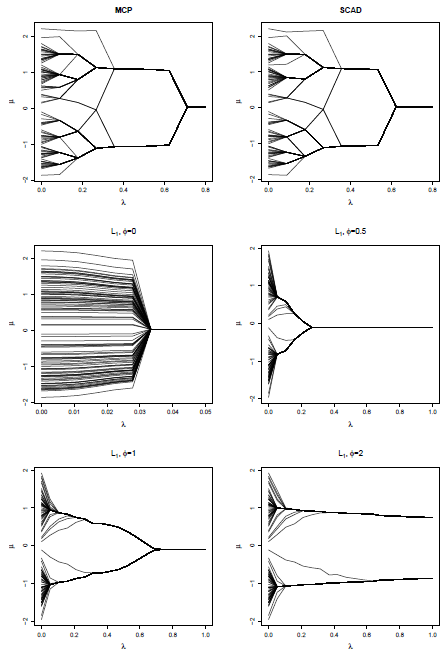
\includegraphics[width=.8\textwidth]{solution_path.png}
\end{figure}

From Table \ref{tab:1}, we compare the results of two algorithms in different computing environments. Our two-step fusion penalty distributed algorithm applies in data distributed storage computing environment, and the concave pairwise fusion approach applies in stand-alone environment. In order to study the influence of the space separation data storage on estimation, we set the same sample size. The difference in comparison is that in distributed environment, data is stored distributed in M nodes, and data of different nodes can not interact. In the stand-alone environment, all data are stored on a single computer. The results in Table \ref{tab:1} show that our algorithm can basically solve the problem of data space separation. The accuracy of the results obtained by our algorithm in distributed environment is comparable to that obtained by the concave pairwise fusion approach in single computer.
\begin{table}[H]
	\centering
	\fontsize{5.5}{6}\selectfont
	\begin{threeparttable}
		\caption{The mean, median and standard error (s.e.) of $\hat{K}$ by the MCP, SCAD and weighted $L_1$ based on 100 realizations with n = 100 in distributed and stand-alone environment}
		\label{tab:1}
		\begin{tabular}{ccccccccccc}
			\toprule
			\multirow{2}{*}{$c$}&\multirow{2}{*}{Method}&
			\multicolumn{3}{c}{ $\alpha=1$}&\multicolumn{3}{c}{$\alpha=1.5$}&\multicolumn{3}{c}{$\alpha=2$}\cr
			\cmidrule(lr){3-5} \cmidrule(lr){6-8}\cmidrule(lr){9-11}
			&&mean&median&s.e.&mean&median&s.e.&mean&median&s.e.\cr
			\midrule
			\multirow{8}{*}{$5$}&MCP&&&&&&&&&\cr
			&DisMCP&&&&&&&&&\cr
			&SCAD&&&&&&&&&\cr
			&DisSCAD&&&&&&&&&\cr
			&$L_1(\phi=1)$&&&&&&&&&\cr
			&Dis$L_1(\phi=1)$&&&&&&&&&\cr
			&$L_1(\phi=2)$&&&&&&&&&\cr
			&Dis$L_1(\phi=2)$&&&&&&&&&\cr
			\midrule
			\multirow{8}{*}{$10$}&MCP&&&&&&&&&\cr
			&DisMCP&&&&&&&&&\cr
			&SCAD&&&&&&&&&\cr
			&DisSCAD&&&&&&&&&\cr
			&$L_1(\phi=1)$&&&&&&&&&\cr
			&Dis$L_1(\phi=1)$&&&&&&&&&\cr
			&$L_1(\phi=2)$&&&&&&&&&\cr
			&Dis$L_1(\phi=2)$&&&&&&&&&\cr
			\bottomrule
		\end{tabular}
	\end{threeparttable}
\end{table}
\begin{table}[H]
	\centering
	\fontsize{5.5}{6}\selectfont
	\begin{threeparttable}
		\caption{The mean and standard error (s.e.) shown in parentheses of the square root of the MSE for the estimated values of $\mu$ and $\beta$ by the MCP, SCAD and $L_1$ penalty based on 100 realizations with n=100 and M=5}
		\label{tab:2}
		\begin{tabular}{cccccccc}
			\toprule
			\multirow{2}{*}{$c$}&\multirow{2}{*}{Method}&
			\multicolumn{3}{c}{ $\mu$}&\multicolumn{3}{c}{$\beta$}\cr
			\cmidrule(lr){3-5} \cmidrule(lr){6-8}
			&&$\alpha=1$&$\alpha=1.5$&$\alpha=2$&$\alpha=1$&$\alpha=1.5$&$\alpha=2$\cr
			\midrule
			\multirow{8}{*}{$5$}&\multirow{2}{*}{MCP}&&&&&&\cr
			&&&&&&&\cr
			&\multirow{2}{*}{SCAD}&&&&&&\cr
			&&&&&&&\cr
			&\multirow{2}{*}{$L_1(\phi=1)$}&&&&&&\cr
			&&&&&&&\cr
			&\multirow{2}{*}{$L_1(\phi=2)$}&&&&&&\cr
			&&&&&&&\cr
			\midrule
			\multirow{8}{*}{$10$}&\multirow{2}{*}{MCP}&&&&&&\cr
			&&&&&&&\cr
			&\multirow{2}{*}{SCAD}&&&&&&\cr
			&&&&&&&\cr
			&\multirow{2}{*}{$L_1(\phi=1)$}&&&&&&\cr
			&&&&&&&\cr
			&\multirow{2}{*}{$L_1(\phi=2)$}&&&&&&\cr
			&&&&&&&\cr
			\bottomrule
		\end{tabular}
	\end{threeparttable}
\end{table}
\section{Real data example}\label{sec:5}
In this section, we use the Cleveland Heart Disease Dataset to illustrate our method. The Cleveland Clinic Foundation heart disease dataset, contributed to the respository by Robert Detrano, contains 303 observations, 165 of which describe healthy people and 138 sick ones; 7 observations are incomplete, and 2 of the observations of healthy people have identical attribute values. We take the complete observation in our analysis. Each observation is described by 13 attributes, including 3 Boolean(e.g. sex), 4 nominal(e.g. type of chest pain), and 6 numerical(e.g. age). The output indicates the angiographic status of the disease, i.e. whether the narrowing of the vessel diameter is above or below 50\%. Our analysis is to conduct subgroup for the fitted value of thalach as the response $y$ after adjusting for the effects of the covariates: $x_1$=age in year; $x_2$=gender; $x_3$=resting blood pressure; $x_4$=serum cholesterol; $x_5$=fasting blood suger indicator; and $x_6$=resting electrocardiographic result;

In order to simulate hospital data sharing, we artificially distribute the samples in 5 nodes. We fit the heterogeneous model \ref{equ:1}, and we identify subgroups by our proposed two-step fusion penalty approach. We select the tuning parameter by minimizing the modified BIC. As a result, two major groups are identified by both of the MCP and SCAD methods.
\begin{table}[H]
	\centering
	\fontsize{5.5}{6}\selectfont
	\begin{threeparttable}
		\caption{The estimated values (est) for the coefficients $\beta$ and $\mu$ by the OLS, MCP and SCAD under stand-alone and distributed environment}
		\label{tab:3}
		\begin{tabular}{ccccccccc}
			\toprule
			Method&$\beta_1$&$\beta_2$&$\beta_3$&$\beta_4$&$\beta_5$&$\beta_6$&$\mu_1$&$\mu_2$\\
			\midrule
			OLS&&&&&&&-&-\\
			MCP&&&&&&&&\\
			DisMCP&&&&&&&&\\
			SCAD&&&&&&&&\\
			DisSCAD&&&&&&&&\\
			\bottomrule
		\end{tabular}
	\end{threeparttable}
\end{table}
We also calculate the coefficient of determination $R^2$, and obtain $R^2$ = \textcolor{red}{XXX,XXX,XXX,XXX and XXX} for MCP, DisMCP, SCAD, DisSCAD and OLS methods. We see that taking into account the subgroup structure leads to a significant improvement of the model fitting. We find that for the actual data, even if we artificially distribute them in different nodes, the results obtained by our approach are almost the same as those obtained by concave pairwise fusion approach in a single computer environment.
\section{Conclusion}
The continued push for nationwide interoperability has helped fuel the growth of secure healthcare data sharing. Covered entities and business associates are exploring how to enhance patient care by engaging in health information exchange (HIE). Genetic studies,  population health management, larger-scale analytics are some potential uses for data sharing. On the other hand, with the continuous development of industry, individual medical has become an inevitable trend. We focus on how to make individual medical care more accurate on the premise of HIE. In this paper, we propose a distributed algorithm named two-step fusion penalty approach to estimate the heterogeneous treatment effects under distributed storage. Our method allows us to ignore the impact of data storage separation when calculating heterogeneous effects. At the same time, our algorithm guarantees the computational efficiency because of its minimal interactive consumption. In the numerical simulation, we find that our algorithm in the distributed storage environment performs almost as well as concave pairwise fusion approach in stand-alone environment. As an application, we analysis the Cleveland heart disease dataset and we see that our approach leads to a significant improvement of the model fitting. The related package 2FusPen are available at ...
\section{Appendix}
In this Appendix, we describe the detail derivation of some updated computations in detailed algorithm \ref{alg:2}. For simplicity of calculation, we set $a_{ij}=a$.
\subsection{Update $\mu^{(k+1)}$ and $\beta^{(k+1)}$}
Hence 
$$
\begin{aligned}
L=&\frac{1}{2}\sum_{i=1}^n(y_i-\mu_i-X_i^T\beta)^2+\sum_{1\leq i<j\leq n}P(|\eta_{ij}|,\lambda)\\
&+\sum_{1\leq i<j\leq n}(\frac{a_{ij}}{2}\lVert \mu_i-\mu_j-\eta_{ij}\rVert+<\mu_i-\mu_j-\eta_{ij}, v_{ij}>)
\end{aligned}
$$
which implies
$$
\mu^{(k+1)}=\arg\min_{\mu}\left\{\frac{1}{2}\sum_{i=1}^n(y_i-\mu_i-X_i^T\beta)^2+\sum_{1\leq i<j\leq n}(\frac{a_{ij}}{2}\lVert \mu_i-\mu_j-\eta_{ij}\rVert+<\mu_i-\mu_j-\eta_{ij}, v_{ij}>)\right\}.
$$
...
$$
\mu^{(k+1)}=(I+a\Delta^T\Delta-Q_X)^{-1}\left\{(I-Q_X)y+a\Delta^T(\eta^{k}-a^{-1}v^{(k)})\right\},
$$
where $Q_X=X(X^TX)^{-1}X^T$, $\Delta=\left\{(e_i-e_j), i<j\right\}^T$ and $e_i$ is the $i$th unit $n\times 1$ vector whose $i$th element is 1 and the remaining ones are 0.

$$
\beta^{(k+1)}=(X^X)^{-1}X^T(y-\mu^{k+1})
$$
\subsection{Update $\eta^{(k+1)}$}
Let $\delta_{ij}=\mu_i-\mu_j+a^{-1}v_{ij}$ and $ST(t,\lambda)=sign(t)(|t|-\lambda)_+$
$L_1$ penalty:
$$\hat{\eta}_{ij}=ST(\delta_{ij},\lambda/a)$$
MCP:
$$
\hat{\eta}_{ij}=\left\{
\begin{array}{lcl}
\frac{ST(\delta_{ij},\lambda/a)}{1-1/(\gamma a)}&&if |\delta_{ij}|\leq \gamma\lambda\\
\delta_{ij}&&if |\delta_{ij}|>\gamma\lambda
\end{array}
\right.
$$
SCAD:
$$
\hat{\eta}_{ij}=\left\{
\begin{array}{lcl}
ST(\delta_{ij},\lambda/a)&&if|\delta_{ij}|\leq\lambda+\lambda/a\\
\frac{ST(\delta_{ij},\gamma\lambda/((\gamma-1)a))}{1-1/((\gamma-1)a)}&&if \lambda+\lambda/a<|\delta_{ij}|\leq \gamma\lambda\\
\delta_{ij}&&if |\delta_{ij}|>\gamma\lambda
\end{array}
\right.
$$
\section*{References}

\bibliography{mybibfile}

\end{document}